%! Author = joels
%! Date = 24/12/2020

\section{Dynamic Polymorphism}
% You can safely employ virtual dispatch
% You can explain the dangers when working with value semantics and dynamic dispatch
% You can use virtual base classes with std::unique_ptr

\subsubsection{Reasons for using Inheritance}
\begin{itemize}
    \item Mix-in functionality from empty base class
    \begin{itemize}
        \item Often with own class as template argument
        \item No inherited data members, only added functionality
    \end{itemize}
\end{itemize}
\begin{lstlisting}[style=frame, style= linenumbers, language=C]
struct Date : boost::equality_comparable<Date> {
    // ...
}
\end{lstlisting}

\vspace{1em}

\begin{itemize}
    \item Adapting concrete classes
    \begin{itemize}
        \item No additional own data members
        \item Convenient for inheriting member functions and constructors
    \end{itemize}
\end{itemize}
\begin{lstlisting}[style=frame, style= linenumbers, language=C]
template<typename T, typename Compare>
struct indexableSet : std::set<T, Compare> {
    // ...
}
\end{lstlisting}

\subsubsection{Inheritance for dynamic binding}
\begin{itemize}
    \item Implementing a design pattern with dynamic dispatch
    \begin{itemize}
        \item Provide common interface for a variety of dynamically changing or different implementations
        \item Exchange functionality at run-time
    \end{itemize}
    \item Base class/interface provides a common abstraction that is used by clients
\end{itemize}
\begin{center}
    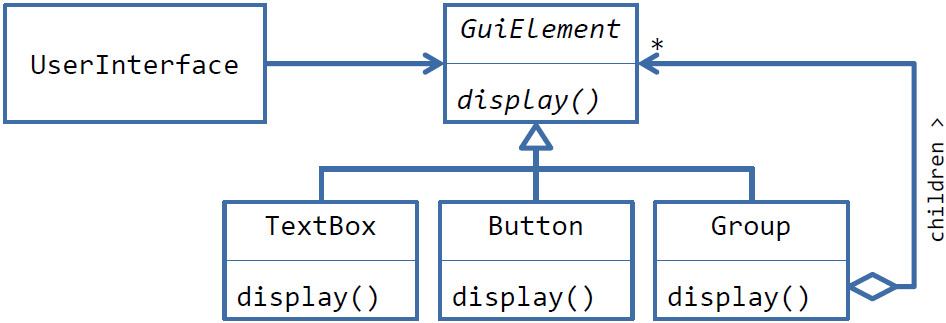
\includegraphics[width=0.6\linewidth]{inheritance_for_dynamic_binding.png}
\end{center}

\subsection{Inheritance Syntax}
\begin{itemize}
    \item Inherit class: default private
    \item Inherit struct: default public
    \item \textit{public}-Keyword: public Base class
    \item \textit{private}-Keyword: private Base struct
    \item Multiple Bases: Sequence is important (Reihenfolge)
    \item With interface inheritance, base class must be public
\end{itemize}

\begin{lstlisting}[style=frame, style= linenumbers, language=C]
class Base {};
struct Base2 {};
class DerivedPrivateBase : Base {}; // private -> class
class DerivedPublicBase : public Base {}; // public -> public keywork
struct DerivedPublicBase : Base {}; // public -> struct
struct MultipleBases : public Base, private Base2 {}; // Multiple Bases
\end{lstlisting}

\pagebreak

\subsubsection{Initializing multiple base classes}
\begin{itemize}
    \item Base constructors can be explicitly called in the member initializer list
    \item You should put base class constructor before the initialization of members
\end{itemize}

\begin{lstlisting}[style=frame, style= linenumbers, language=C]
class DerivedWithCtor : public Base1, public Base2 {
    int mvar;
public:
    DerivedWithCtor(int i, int j) :
        Base{i}, Base2{}, mvar{j} {}
};
\end{lstlisting}


\subsection{Dynamic polymorphism}
\begin{itemize}
    \item Operator and function overloading and templates allow polymorphic behaviour at compile time
    \item Dynamic polymorphism needs object references or (smart) pointers to work
    \begin{itemize}
        \item Syntax overhead
        \item The base class must be a good abstraction
        \item Copying carries the danger of slicing (partially copying)
    \end{itemize}
\end{itemize}

\subsubsection{Shadowing Member Functions}
\begin{itemize}
    \item if a function is reimplemented in a derived class, it shadows its counterpart in the base class
    \item However, if accessed through a declared bases object, the shadowing function is ignored
\end{itemize}

\begin{lstlisting}[style=frame, style= linenumbers, language=C]
struct Base {
    // shadowed function
    void sayHello() const {
        std::cout << "Hi, I'm Base\n";
    }
};

struct Derived : Base {
    // shadowing function
    void sayHello() const {
        std::cout << "Hi, I'm Derived\n";
    }
};

void greet(Base const & base) {
    base.sayHello();
}

int main() {
    Derived derived{};
    greet(derived); // Hi, I'm Base (static call)
}
\end{lstlisting}

\pagebreak

\subsubsection{Virtual Member Functions}
\begin{itemize}
    \item Dynamic polymorphism requires base classes with \textit{virtual} member functions
    \item \textit{virtual} Member functions are bound dynamically
\end{itemize}

\begin{lstlisting}[style=frame, style= linenumbers, language=C]
struct Base {
    virtual void sayHello() const {
        std::cout << "Hi, I'm Base\n";
    }
};

struct Derived : Base {
    virtual void sayHello() const {
        std::cout << "Hi, I'm Derived\n";
    }
};

void greet(Base const & base) {
    base.sayHello();
}

int main() {
    Derived derived{};
    greet(derived); // Hi, I'm Derived (dynamic call)
}
\end{lstlisting}

\subsubsection{Overriding virtual Member Functions}
\begin{itemize}
    \item \textit{virtual} is inherited and can be omitted in the derived calss
    \item It is possible to mark an overriding function with \textit{override}
\end{itemize}

\begin{lstlisting}[style=frame, style= linenumbers, language=C]
struct Derived : Base {
    void sayHello() const override {
        std::cout << "Hi, I'm Derived\n";
    }
};
\end{lstlisting}

\subsubsection{Signatures when Overriding}
\begin{itemize}
    \item To override a virtual function in the base class the signature must be the same
    \item constness of the member function belongs to the signature
\end{itemize}

\subsubsection{Calling virtual Member functions}
\begin{itemize}
    \item Value Object
    \begin{itemize}
        \item Class type determines function, regarless of virtual
    \end{itemize}
    \item Reference
    \begin{itemize}
        \item Virtual member of derived class called through base class reference
    \end{itemize}
    \item Smart Pointer
    \begin{itemize}
        \item Virtual member of derived class called through smart pointer to base class
    \end{itemize}
    \item Dumb Pointer (rarely used)
    \begin{itemize}
        \item Virtual member of derived class called through base class pointer
    \end{itemize}
\end{itemize}

\begin{lstlisting}[style=frame, style= linenumbers, language=C]
// Value Object
void greet(Base base) {
    // always calls Base::sayHello
    base.sayHello();
}

// Reference
void greet(Base const & base) {
    // calls sayHello() of the actual type
    base.sayHello();
}

// Smart Pointer
void greet(std::unique_ptr<Base> base) {
    // calls sayHello() of the actual type
    base->sayHello();
}

// Dump Pointer
void greet(Base const * base) {
    // calls sayHello() of the actual type
    base->sayHello();
}
\end{lstlisting}

\subsubsection{Abstract Base Classes: Pure Virtual}
\begin{itemize}
    \item There are no Interfaces in C++
    \item A pure virtual member function makes a class abstract
    \item To mark a virtual member function as pure virtual it has zero assigned after its signature
    \item Abstract classes cannot be instantiated (like in Java)
\end{itemize}

\begin{lstlisting}[style=frame, style= linenumbers, language=C]
struct AbstractBase {
    virtual void doitnow() = 0;
};
\end{lstlisting}

\subsubsection{Destructors (virtual)}
\begin{itemize}
    \item Classes with virtual members require a virtual Destructor
    \item Otherwise when allocated on the heap with \textit{make\_unique} and assigned to a \textit{unique\_ptr} only the destructor of Base is called
\end{itemize}

\begin{lstlisting}[style=frame, style= linenumbers, language=C]
struct Fuel {
    virtual void burn () = 0;
    virtual ~Fuel() { std::cout << "put into trash\n"; }
};

struct Plutonium : Fuel {
    void burn () { std::cout << "split core\n"; }
    ~Plutonium() { std::cout << "store many years\n"; }
}

int main() {
    // Both destructors called
    std::unique_ptr<Fuel> surprise = std::make_unique<Plutonium>();
}
\end{lstlisting}

\subsubsection{Why Inheritance can be bad}
\begin{itemize}
    \item Very strong coupling between subclass and base class
    \item You can hardly change the base class
    \item API of base class must fit for all subclasses (hard)
\end{itemize}


\subsubsection{Problem with Inheritance and Pass-by-Value}
\begin{itemize}
    \item Assigning or passing by value a derived class value to a base class variable/parameter incurs object slicing
    \item Only base class member variables are transferred
\end{itemize}

\begin{lstlisting}[style=frame, style= linenumbers, language=C]
// Pass-by-Value (slicing of derived object)
void modifyAndPrint(Base base) {
    base.modify();
    base.print(std::cout);
}

int main() {
    Derived derived{25};
    // reduces the derived object to its base (sliced)
    modifyAndPrint(derived);
}
\end{lstlisting}

\pagebreak

\subsubsection{Problems with Member Hiding}
\begin{itemize}
    \item Member functions in derived classes hide base class member with the same name, even if different parameters are used
    \item By \textit{using [member]}, the hidden member becomes visible
\end{itemize}

\begin{lstlisting}[style=frame, style= linenumbers, language=C]
struct Base {
    int member{};
    explicit Base(int initial);
    virtual ~Base() = default;
    // hidden
    virtual void modify();
};

struct Derived : Base {
    using Base::Base;
    // using Base::modify; <-- resolves hiding issue

    // hides base function
    void modify(int value) {
        member += value;
    }
};

int main() {
    Derived derived{25};
    derived.modify(); // Error, base function hidden
}
\end{lstlisting}

\subsubsection{Prevent Object Slicing in Base Class}
\begin{itemize}
    \item Declare the copy operations as deleted
\end{itemize}

\begin{lstlisting}[style=frame, style= linenumbers, language=C]
struct Base {
    Base & operator=(Base const & other) = delete;
    Book(Book const & other) = delete;
}
\end{lstlisting}

\subsubsection{Guidelines}
\begin{itemize}
    \item Only apply inheritance and virtual members if you know what you do
    \item Do not create classes with virtual members by default
    \item Follow the Liskov Substitute Principle
    \begin{itemize}
        \item Base class states must be valid for subclasses
        \item Do not break invariants of the base class
        \item Don't change semantics unexpectedly
        \item \textit{If it looks like a duck and quacks like a duck but needs batteries, you probably have the wrong abstraction.\"}
    \end{itemize}
\end{itemize}